\documentclass[a4paper]{article}

\usepackage[english]{babel}
\usepackage[utf8]{inputenc}
\usepackage{amsmath}
\usepackage{graphicx}
\usepackage[colorinlistoftodos]{todonotes}
\usepackage[useregional]{datetime2}
\usepackage{fancyhdr}
\usepackage{titlesec}
\usepackage{listings} 
\usepackage[hidelinks]{hyperref}
\usepackage{caption}
\usepackage{titling}
\usepackage{varwidth}

\usepackage{color}

\setcounter{secnumdepth}{4}

\setlength{\droptitle}{-4em}

\graphicspath{{../img/}}

%Project Title
\newcommand{\projectTitle}{Make A Movie}
%Homework Number
\newcommand{\hwNumber}{4}

%Submission date goes here.
%Format: #Day of Month #Hour:#Minute AM/PM
\newcommand{\projectDate}{11th of May 11:59 PM}

%Contact to reach.
\newcommand{\contactName}{Kaan Yıldırım}
\newcommand{\contactMail}{kyildirim14@ku.edu.tr}

%Define colors as shown below to use in text.
\definecolor{Red}{RGB}{255, 0, 0}
\definecolor{Green}{RGB}{0, 255, 0}
\definecolor{Blue}{RGB}{0, 0, 255}

\title{\projectTitle\vspace{-2em}}

\date{Submission Date: \projectDate}

\begin{document}
	\maketitle
	
	\lstset{language=Java}
	\pagestyle{fancy}
	\fancyhf{}
	\chead{\projectTitle}
	\rhead{Homework \#\hwNumber}
	\lhead{COMP 130}
	\lfoot{\nouppercase{\leftmark}}
	\rfoot{Page \thepage}
	\thispagestyle{fancy}
	\renewcommand{\headrulewidth}{0.4pt}
	\renewcommand{\footrulewidth}{0.4pt}
	
	\section{Introduction}
	
	\subsection{Submission}
	Submit a \textbf{folder} that is \textbf{only} containing your Java source files (*.java) to the course's Homework folder. 
	\\
	
	Full path: \textbf{F:\textbackslash COURSES\textbackslash UGRADS\textbackslash COMP130\textbackslash Homework\textbackslash}
	\\
	
	\noindent \textbf{Note:} MAVA 130 students, please submit to the folder under the COMP 130 directory.
	\\
	
	\noindent Please use the following naming convention for the submitted folders: \linebreak
	
	\textbf{YourPSLetter\_CourseCode\_Surname\_Name\_HWNumber\_Semester}
	\\
	
	\noindent Example folder names:
	\begin{itemize}
		\item \textbf{PSA\_COMP130\_Surname\_Name\_HW\hwNumber\_S18}
		\item \textbf{PSB\_MAVA130\_Surname\_Name\_HW\hwNumber\_S18}
	\end{itemize}
	
	\noindent Additional notes:
	\begin{itemize}
		\item Using the naming convention properly is important, failing to do so may be \textbf{penalized}.
		\item \textbf{Do not} use Turkish characters when naming files or folders.
		\item Submissions with unidentifiable names will be \textbf{disregarded} completely. (ex. "homework1", "project" etc.) 
		\item Please write your name into the Java source file where it is asked for.
	\end{itemize}
	
	\subsection{Academic Honesty}
	Koç University's \emph{\href{https://vpaa.ku.edu.tr/sites/vpaa.ku.edu.tr/files/Misc_Documents/Statement_on_Academic_Honesty.pdf}{Statement on Academic Honesty}} holds for all the homeworks given in this course. Failing to comply with the statement will be penalized accordingly. If you are unsure whether your action violates the code of conduct, please consult with your instructor.
	
	\subsection{Aim of the Project}
	In this project you are expected to create a \emph{\href{https://en.wikipedia.org/}{Command Line Interface}} (CLI) that will allow the user to create animations. This project also expects you to display the created animation to the user. Your program must be able to save and load animation files.
	
	%Do not change this section.
	\subsection{Given Code}
	This part is \textbf{optional} but advised as it will allow you to understand the given partitions of the code better. \textbf{Do not} change anything in the code if it is indicated to you with a comment. The code given to you has something called \textbf{JavaDoc} comments above all the methods. These comments allow you to view various information about the method when you mouse over the name of the method. Below are the methods given to you in the code with their explanation.
	
	\subsubsection{Given Methods}
	
	\begin{itemize}

		\item \lstinline{void init()}
		
		This is the default initializer for the \lstinline{acm.GraphicsProgram}. It is guaranteed to run before the \lstinline{run()} method. In this project, this method is used to print the welcome message to the console. Do \textbf{not} modify this method.
		
		\item \lstinline{void run()}
		
		This is the entry point for your program. Feel free to modify it as you wish.
		
		\item \lstinline{int generatePixelFromColor(int pixel, Color c)} 
		
		This method converts a given pixel to the given color. This is used to preserve the original alpha value of the pixel. You are not required to use this method, however should you choose not to use it, you are still expected to preserve the alpha values of the pixels.
		
		\item \lstinline{Color generateColorFromString(String str)} 
		
		This method returns a \lstinline{Color} object associated with a given \lstinline{String} value. You can use this method to convert a \lstinline{String} to a \lstinline{Color} to recolor an image.
		
		
	\end{itemize}
	
	\subsubsection{Given Constants}
	Constants are given at the bottom of the project. All constants provide \textbf{JavaDoc} comments above them. Please read these to understand what constant is used for what. \textbf{Do not} use another variable or a static value for something if there is a constant variable defined for that purpose.
	
	\subsection{Further Questions}
	For further questions \textbf{about the project} you may contact \textbf{\contactName} at \href{mailto:\contactMail}{\mbox{[\contactMail]}}. Note that it may take up to 24 hours before you receive a response so please ask your questions \textbf{before} it is too late. No questions will be answered when there is \textbf{less than two days} left for the submission.
	
	\section{Project Tasks}
	\label{tasks}
	The project tasks are divided into subsections to make it easier to understand and implement. You are strictly advised to follow the given order of tasks, however should you choose not to follow the tasks in order, it is possible to implement the project in any order.
	
	\subsection{Creating a Command Line Interface}
	A Command Line Interface (CLI) is a means of interacting with a program where the user issues commands in the form of successive lines of texts. In this task you are expected to create a simple CLI that needs to be capable of recognizing the following commands:
	\label{commands}
	\begin{itemize}
		\item create: Creates a new project.
		\item open: Opens an existing project.
		\item settitle: Sets the title for the project.
		\item setgrammar: Sets the grammar for the project.
		\item addscene: Adds a scene to the current project.
		\item removescene: Removes a scene from the current project.
		\item listscenes: Lists all the scenes in the project.
		\item play: Plays the scenes in order.
		\item save: Saves the project to a file.
		\item close: Closes a project.
		\item quit: Quits the program.
		\item help: Display additional information.
	\end{itemize}
	
	\subsubsection{Building a Basic CLI}
	
	In its most basic form a CLI reads the user input as a string and parses it to call different commands according to the input text. You may want to start by implementing a simple code that asks for user input continuously. Once you have accomplished this, try detecting the input text of "quit". Modify your code so that it asks for a new input from the user as long as the input is not "quit". \\

	\noindent \textbf{Advice:} You may want to echo (print back to the screen) the input you receive from the user to clearly see that you can read the input.
	
	\subsubsection{Detecting All Commands}
	
	Now that you have a basic CLI that is capable of recognizing a specific input, you can proceed by detecting all the commands shown in Section \ref{commands}. You may modify the names of the commands, however you are \textbf{required} to state all the changes when the "help" command is called. Note that as you implement the tasks below, you are expected to link them to these commands. \\
	
	\noindent \textbf{Advice:} You can implement temporary methods for all the commands you have detected and for now print a text that states the command is executed properly.
	
	\subsubsection{Distinguishing Commands From Output}
	
	If you have implemented the suggested way of checking your CLI, you may have noticed that the input and the output lines are mixing up. To prevent this confusion you are expected to print a constant string before taking an input from the user. This is the string defined as \textbf{CLI\_INPUT\_CONST} in the given code.

	\subsection{Creating a New Project}
	In this task you will create a new project from scratch. To be able to achieve this, you need to first understand the animation file format. Below, you can find an example valid project file.
	\label{example}
	\begin{center}
	\fcolorbox{lightgray}{white}{\begin{varwidth}{\textwidth}
		Title New Movie
		
		Images ball tree
		
		Grammar time color image from to
		
		Scenes
		
		For 5 seconds red ball from left to right
		
		For 1500 milliseconds green tree from bottom to top
		
	\end{varwidth}}	
	\end{center}

	
	The first line always starts with the keyword \textbf{Title} and is followed by the title of the animation. Note that the animation title is not necessarily a single word. The second line always starts with the keyword \textbf{Images} and is followed by the name of all image files that are going to be used in the animation. The third line always starts with the keyword \textbf{Grammar} and is followed by the grammar specification of the animation. The fourth line is the keyword \textbf{Scenes} which is followed by scene descriptions, one per line. The scene descriptions are required to follow the grammar.\\
	
	The grammar allows the user to change the way they want to describe the scene. As a real world example, you can see that Turkish and English have different grammars. Below is a list of all grammar descriptors defined for this project.
	\label{grammar}
	\begin{itemize}
		\item color: A single word describing a color. Example: red
		\item image: A single word that is the name of a image file. Example: plan
		\item from: A two word descriptor that starts with the keyword \textbf{from} and is followed by a location. Example: from left
		\item to: A two word descriptor that starts with the keyword \textbf{to} and is followed by a location. Example: to right
		\item time: A three word descriptor that starts with the keyword \textbf{for} and is followed by an integer value which is followed by either the word \textbf{second(s)} or \textbf{millisecond(s)}.
	\end{itemize}

	\noindent \textbf{Note:} The locations described in the \textbf{from} and \textbf{to} descriptors can take the following values: left, right, top, bottom, center.
	
	\begin{figure}[!htb]
		\centering
		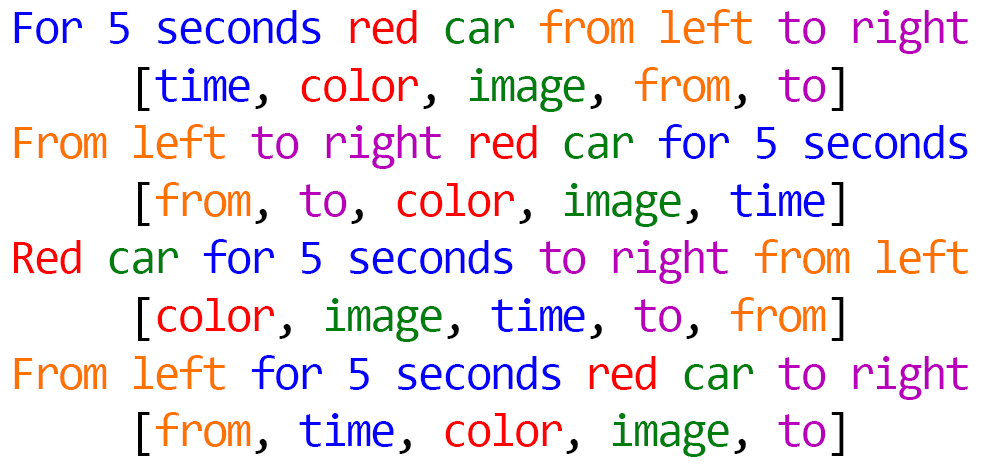
\includegraphics[width=0.8\textwidth]{../img/example_grammar.png}
		\caption{An example scene description according to multiple different grammars. Descriptors of the same type are colored in the same color. Grammar specified for each scene resides below it.}
	\end{figure}
	
	\subsubsection{Creating a New Project, Actually.}
	
	In this task you are required to start implementing the commands that your CLI can detect. Start with the \textbf{create} command, which is expected to ask the user for a new project name. (Note that this is different from the project title.) Once you get this name for the project, modify your CLI so that it displays this name before the \textbf{CLI\_INPUT\_CONST} seperated with a '@' character. \\
	
	\noindent Example for project name TestProject: \textbf{TestProject@MakeAMovie -\textgreater}\\
	
	Now that you have created a new project (not yet, really) you may also implement the \textbf{settitle} command. This command will ask the user for a title, later on you will be expected to save these to a file so please make sure that you do not lose any information the user inputs.\\
	
	Once you achieved getting the title from the user, you may proceed with the \textbf{setgrammar} command. This command will take the ordering of the grammar descriptors defined in Section \ref{grammar} from the user. You will later on use this to parse the animation scenes.\\
	
	\noindent \textbf{Hint:} You may want to save the grammar to either a string, an array of strings or something else as it is later on required. \\
	
	As you have acquired the grammar specification, you may now allow the user to start inputting new scenes. Implement the \textbf{addscene} command so that the user can add a scene by describing it according to the grammar that they defined. This command will read a \textbf{single} line of user input. \\
	
	\noindent \textbf{Hint:} String class has a method \lstinline{split(String str)} which splits the string it is \textbf{called on} and returns an array of strings that were originally separated by str. (Example: \lstinline{"This-is-a-test-string".split("-")} will return a string array of \{"This", "is", "a", "test", "string"\}) Note that the string the method is called on can be a variable as well. \\
	
	After an excessive usage of \textbf{addscene} command a user may lose track of the scenes added, and may want to see what is currently in the project. At this point you are expected to implement the \textbf{listscenes} command that will list all the current scenes in order, starting their enumeration from 1. (Meaning the first scene is the scene number 1) \\
	
	\begin{center}
		\fcolorbox{lightgray}{white}{\begin{varwidth}{\textwidth}
				1) For 5 seconds red ball from left to right
				
				2) For 1500 milliseconds green tree from bottom to top
				
		\end{varwidth}}	
	\end{center}
	\emph{An example output from \textbf{listscenes} command that shows how the enumeration works.}\\
	
	Once seeing all the scenes present in the project, a user may want to remove a scene from the animation. Notice how you enumerated the scenes in the \textbf{listscenes} command, you are now required to implement \textbf{removescene} command. This command will ask the user to input a scene number, and will remove it from the project. After a removal, the enumeration of the scenes may change if the scene removed was not the last scene. (In an animation with four scenes, the removal of second scene would make the third the second and the fourth the third.) \\
	
	\subsubsection{Saving and Loading a Project}

	While testing your program you may have noticed that it is annoying to reenter all the information about a project. To solve this problem, you are expected to implement \textbf{save} command. Create a new file using the project name (not project title) and the \textbf{FILE\_TYPE} constant provided. (Note that the FILE\_TYPE is the extension of the file, thus it is required to be at the end of the file name) You are required to save the project information in the same format as provided and explained in Section \ref{example}. \\
	
	Now that you can save your project files, you also need to be able to open them later on using the \textbf{open} command. This command asks the user for a file name and loads the information saved in that file. (Note that the user enters the file name without the FILE\_TYPE)
	
	\subsection{Making Your Film (Where the Magic Happens)}
	Up until now, you worked with the boring infrastructure of the project. Now is the time for you to become the director of your (or maybe someone else's) film! The tasks below will guide you through the process of animating the scenes.
 	
	\subsubsection{Creating an Animation Loop}
	An animation consists of at least one scene. However one scene is hardly enough to express anything meaningful. You may find it beneficial to create a loop that iterates over all the scenes, before starting the animation part itself. In the next task you may simply fill in this loop to actually animate all the scenes.
	
	\subsubsection{Animating the Scenes, Actually}
	Animating a scene is nothing more than extracting meaningful information from the scene according to the grammar and applying your graphics knowledge to it. You are expected to load and recolor the image file in the scene according to the color given in the scene description.\\
	
	Once you obtain a correctly recolored image file, you can add it to the location specified by the \textbf{from} descriptor. Note that you are expected to place the image in the center of the specified location. (i.e. placing an image to the left means that the middle of the left edge of the image must coincide with the middle of the left edge of the screen.)\\
	
	\begin{figure}[!htb]
		\centering
		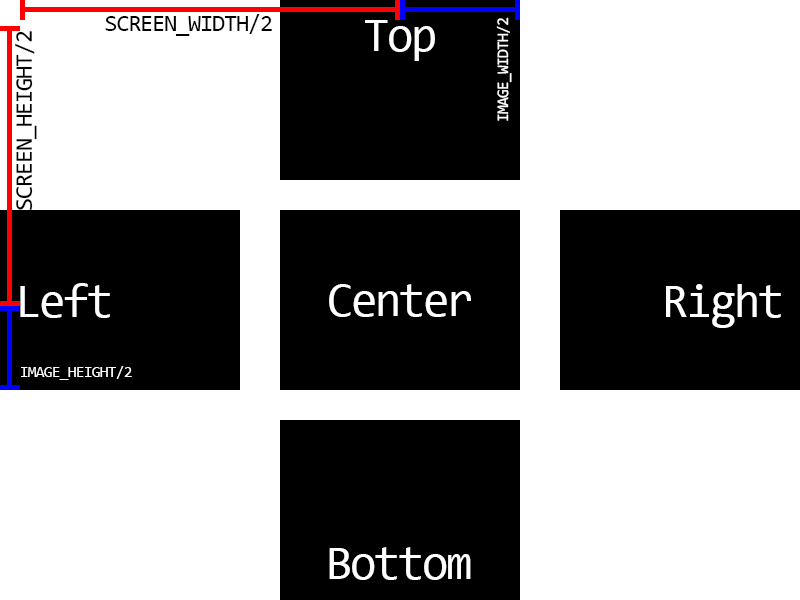
\includegraphics[width=0.8\textwidth]{../img/image_placement.png}
		\caption{Positioning of images according to the locations. Notice how all images are always in the screen.}
	\end{figure}
	
	Now that you have the image on the screen, you need to move it to the location specified by the \textbf{to} descriptor. Note that this movement must be \textbf{uniform} and must take exactly the amount of time specified by the \textbf{for} descriptor.
	
	
	%Do not change this section.
	\subsection{End of Project}
	Your project ends here. You may continue to tinker with the code to implement any desired features and discuss them with your section leader. Below in the \textbf{Section \ref{further}} are further tasks for you to implement if you are willing to continue practicing the topics. However, \textbf{do not} include any additional features that you implement after this point in to your submission.  
	\\
	
	\noindent \textbf{Final Warning: Do not include anything beyond this point to your submission.} 
	
	\newpage
	
	\section{Further Tasks}
	\label{further}
	Tasks described in this section are \textbf{not} included to your project, but are provided for studying the topics further. \textbf{Do not} submit your project with any of these tasks completed. You will only be graded for the tasks in \textbf{Section \ref{tasks}}.

	\subsection{A More Complex Understanding}
	As is, your program is capable of understanding colors that are preset by Java. It can also only understand a given subset of locations defined by you. This however is very restrictive. There are a few things you can implement to extend the capabilities of your program.
	
	\subsubsection{Understanding RGBA}
	Modify your program so that it can \textbf{also} understand a color given the RGBA value in the following format: (R, G, B, A). Notice as you are specifying the alpha value as well, you will need a different way to recolor images.
	
	\subsubsection{Understanding Coordinates}
	Modify your program so that it can \textbf{also} understand a location given the XY value in the following format: (X, Y). When a coordinate is specified in this format, place the center point of the image to the given coordinate.
	
	\subsubsection{Quality Assurance}
	\begin{center}
		\fcolorbox{lightgray}{white}{\begin{varwidth}{\textwidth}
				A QA engineer walks into a bar, and orders a beer.
				
				Then he orders 0 beers.
				
				Then he orders 999999999999 beers.
				
				Then he orders an aardvark.
				
				Then he orders nothing.
				
				Then he orders -1 beers.
				
				Then he orders null beers.
				
				Then he orders asnwikfjsdf.
				
				Finally, the QA engineer leaves without paying,
				
				comes back, and asks for the tab.
		\end{varwidth}}	
	\end{center}

	The excerpt above is a funny analogy of the life of an quality assurance engineer. Programs are tested with a wide range of both sensible and senseless inputs. The goal is to fix the program so that there exists no unexpected behavior. Apply the same procedure to your program and try to handle all the errors that may be caused from illegal inputs. An example of this may be only allowing scenes that are correct according to the given grammar. Another example can be handling an error raised by trying to open an file that does not exist.
	
	
\end{document}